\documentclass[12pt,a4paper]{article}

\usepackage[utf8]{inputenc}
\usepackage{ctex}
\usepackage{amsmath,amsfonts,amssymb}
\usepackage{abstract,appendix}
\usepackage{makeidx,hyperref}
\usepackage{graphicx,epsfig,subfig}
\usepackage{geometry}
\usepackage{xcolor}

\geometry{scale=0.8}

%\setlength{\lineskip}{\baselineskip}
\setlength{\parskip}{0.5\baselineskip}

\title{Anderson局部化实验报告6(补充)}
\author{sis-flag}
\date{\today}

\begin{document}

\maketitle

\subsection*{聚集到边界的程度}

研究特征值问题,定义在$[0,1]^d$上。
\begin{align*}
-\Delta u + K V u = \lambda u \qquad \mathbf{x} \in \Omega \\
\frac{\partial u}{\partial n} + h u = 0 \qquad \mathbf{x} \in \partial \Omega
\end{align*}

研究$V(x)$为Bernoulli分布的情况。\textbf{它以概率$p$取值为0,概率$q=1-p$取值为1。}

一维情况下,对于某个特征函数$u(x)$,定义它聚集到边界的“程度”
为$$ Pb = \frac{\max\{|u(0)|, |u(1)|\}}{\max_{x \in \Omega} |u(x)|} $$

二维情况下,定义它localize到边界的“程度”为
$$ Pe = \frac{\max_{x \in \partial\Omega} |u(x)|}{\max_{x \in \Omega} |u(x)|} $$
同样可以定义localize到角落的“程度”为
$$ Pc = \frac{\max\{|u(0,0)|, |u(0,1)|, |u(1,1)|, |u(1,0)|\}}{\max_{x \in \Omega} |u(x)|} $$

在Dirichlet边界下,这些都是0。在导数边界条件下,随着$V(x)$随机生成,这些量就是一些和$K,p,h$有关的随机变量。取值在0到1之间。下面研究这个随机变量的分布随参数的变化。

这里\textbf{只研究了最小特征值对应的特征函数},其它较小特征值的规律和它是一样的。

\subsection*{理论推导}

根据之前的推断,一维的Neumann边界条件下,$K$很大的时候,特征函数聚集与边界的概率等于“边界上一段取值为0的长度的2倍,大于内部所有取值为0段的长度”这个事件的概率。

假设已经观察到两段取值为$1$和$0$,设后面取值为$0$对应的段数为$X$,$X$是一个随机变量。它取值为$n$的概率等于“在后面观察到$n-1$段为$0$”的概率乘以“在$n$处观察到$1$”的概率。

由于区间总数有限,$X$实际上应该服从一个“截断的几何分布”,在N很大的时候,可以用几何分布近似它
$$ \mathbb{P}(X = n) = p^{n-1} q $$
均值$E(X) = 1/q$。而且
$$ \mathbb{P}(X < n) = 1 - p^{n-1} $$

同理,已经观察到两段取值为0和1,设后面取值为1对应的段数为Y。Y也近似服从几何分布
$$ \mathbb{P}(Y = n) = q^{n-1} p $$
均值$E(Y) = 1/p$

在整个区间中,一个全为0的段和一个全为1的段一定交替出现,称为一个“周期”。每个周期的平均长度为$E(X+Y) = \frac{1}{p q}$。所以整个区间里的平均“周期”数为$N p q$,也就是$2 N p q$个取值相同的段。

设$M = N p q$,在平均的意义下,我们可以近似地认为长度为$X_1, Y_1, \cdots, X_M, Y_M$的取值相同的段组成。(这个假设随着$N$增大不会变准确)

这些随机变量$X_1, Y_1, \cdots, X_M, Y_M$相加要等于$N$,所以它们之间不是独立的。但是在$N$很大的时候,我们近似认为它们独立。

\paragraph*{情况1}
两端取值都为$0$,这种情况出现的概率为$p^2$。

我们所求的概率为
\begin{align*}
  & \mathbb{P}(\max\{X_2, X_3, \cdots, X_{M-1}\} < 2 \max\{X_1, X_M\}) \\
= & \sum_{m,n=1}^{\infty} \mathbb{P}(\max\{X_2, X_3, \cdots, X_{M-1}\} < 2 \max\{m,  n\}) \mathbb{P}(X_1 = m) \mathbb{P}(X_M = n) \\
= & \sum_{m,n=1}^{\infty} [\mathbb{P}(X_i < 2 \max\{m,n\}) ]^{M-2} \mathbb{P}(X_1 = m) \mathbb{P}(X_M = n)\\
= & \sum_{m,n=1}^{\infty} (1 - p^{2 \max\{m,n\}-1})^{M-2} p^{m-1} q p^{n-1} q\\
= & \sum_{k=1}^{\infty} p^{k-2} q^2 \sum_{n=1}^{k-1} (1 - p^{2 \max\{k-n,n\}-1})^{M-2} 
\end{align*}

\paragraph*{情况2}
左边取值为$0$,右边取值为$1$,这种情况出现的概率为$pq$。

我们所求的概率为
\begin{align*}
  & \mathbb{P}(\max\{X_2, X_3, \cdots, X_{M}\} < 2 X_1) \\
= & \sum_{n=1}^{\infty} \mathbb{P}(\max\{X_2, X_3, \cdots, X_{M-1}\} < n) \mathbb{P}(X_1 = n) \\
= & \sum_{n=1}^{\infty} [\mathbb{P}(X_i < 2 n]^{M-1} \mathbb{P}(X_1 = n)\\
= & q \sum_{n=1}^{\infty} (1 - p^{2 n-1})^{M-2} p^{n-1}
\end{align*}

\paragraph*{情况3}
左边取值为$1$,右边取值为$0$,同理。

\subsection*{实验模拟}

首先随机生成一些Bernoulli分布的数,验证概率计算的准确性。预测和模拟的结果比较一致,如图\ref{qk}。这里$N=50$,采样个数为$10000$。
\begin{figure}[h]
\centering
\subfloat[情况1]{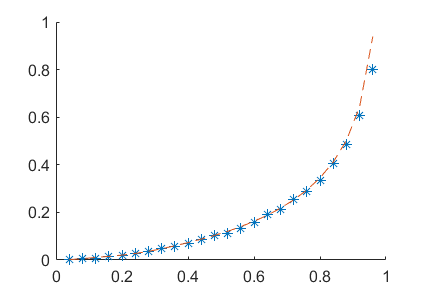
\includegraphics[width=0.3\linewidth]{qk1}}
\subfloat[情况2+3]{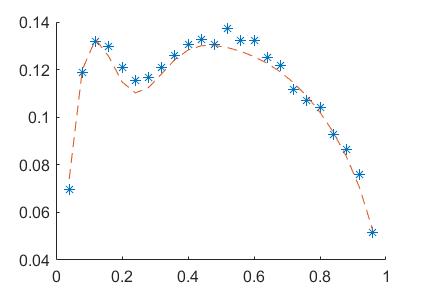
\includegraphics[width=0.3\linewidth]{qk23}}
\subfloat[总体概率]{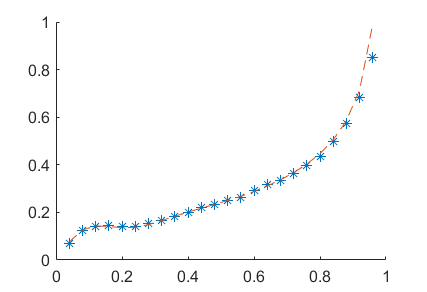
\includegraphics[width=0.3\linewidth]{qka}}
\caption{实验结果(N=50)}
\label{qk}
\end{figure}

这里需要注意的是,$N$的个数不能太小。取$N=20$,重复上面的实验,结果如图\ref{20qk}。在$p$较大的时候不准确,预测值甚至已经大于$1$了。
\begin{figure}[h]
\centering
\subfloat[情况1]{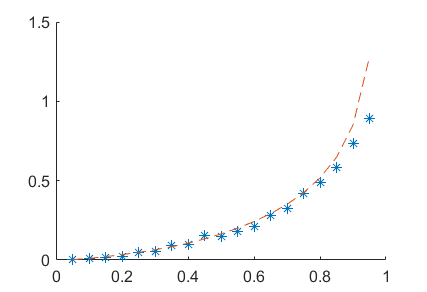
\includegraphics[width=0.3\linewidth]{20qk1}}
\subfloat[情况2+3]{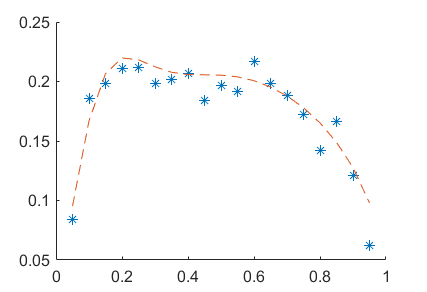
\includegraphics[width=0.3\linewidth]{20qk23}}
\subfloat[总体概率]{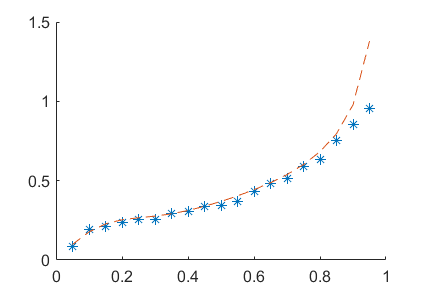
\includegraphics[width=0.3\linewidth]{20qka}}
\caption{实验结果(N=20)}
\label{20qk}
\end{figure}

根据之前的结果,一维的模型中$h$很小,$K$很大时,可以近似为Neumann边界条件。此时,要分两种情况讨论。如果$V(x)$恒为$1$,特征函数就近似是常数,集中到边界的程度为$1$。如果$V(x)$有一段不为$1$,这个时候聚集到边界的程度就由上面计算的概率决定。

全取1的概率为$(1-p)^N$,我们把这一项加到预测值里面,计算聚集到边界的程度。这里参数$h=0.01$,$K=10^4$。图中红色线为模拟得到的$Pb$的均值,紫色线是在相同的样本下计数得到的“最长一段位于边界”的频率。蓝色线是预测值。

\begin{figure}[h]
\centering
\subfloat[N=20]{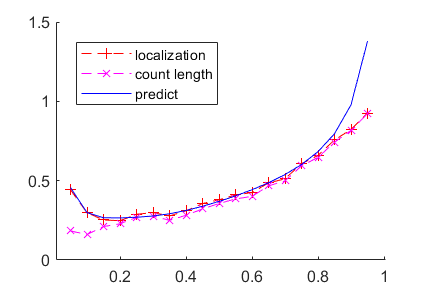
\includegraphics[width=0.3\linewidth]{extra20}}
\subfloat[N=50]{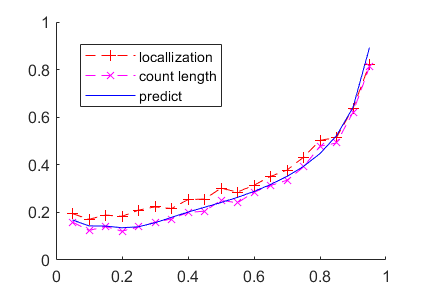
\includegraphics[width=0.3\linewidth]{extra50}}
\caption{实验结果}
\label{extra}
\end{figure}

可以看出,在$N=20$时,$V(x)$恒为1这种情况对应的概率无法忽略,曲线在靠近0的位置会翘起来。$N=50$时,翘起来的程度会更陡峭,图里画不出来。而且$N$较小,$p$靠近1的时候预测不准确,这个也和之前的模拟结果吻合。

\newpage
\subsection*{相变}
这里我们考虑一维的情况。势函数取成:$N_2/2$个1 + $N_1$个0 + $N_2$个1 +  $N_3$个0 +  $N_4$个1 +  $N_5$个0 + :$N_2/2$个1。其中$\max\{N_3, N_5\} < N_1 < N_3 + N_5$(两边差不多长),$N_4 < \min\{N_3, N_5\} / 2$(被吃掉的部分要足够短),$N_2 > N_1+ N_3 + N_4 + N_5$(中间的分隔要足够长)。边界为周期边界。总长度$N = N_2 + N_1 + N_2 + N_3 + N_4 + N_5$。
\begin{figure}[h]
\centering
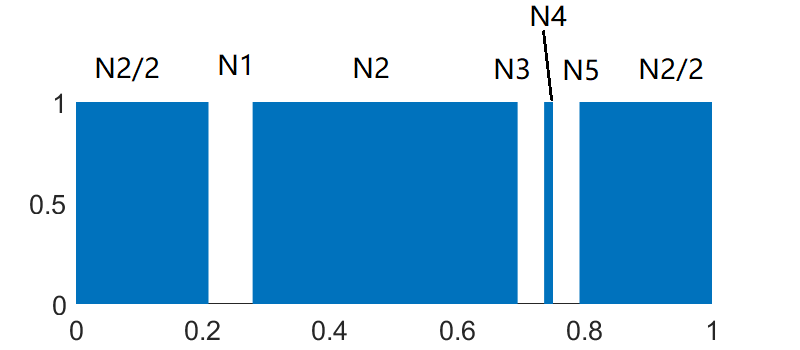
\includegraphics[width=0.7\linewidth]{N}
\caption{示意图}
\end{figure}

\textbf{更新了代码,增加了非均匀网格求解的部分。现在的$N$可以是小数。}

这里对变量进行归一化,考虑$N_3=N_5$的情况,定义
下面分别模拟这些变量和相变点之间的关系。\textbf{在之前的报告里我犯了个错误,在拟合某个变量和其它变量之间关系的时候,并没有保证其它变量不变。控制变量没有控制好。}

这里的4个变量,一共有3个自由度。我们选取要拟合的变量为
$$ L_2 = \frac{N_2}{N_1 + 2 N_2 + N_3 + N_4 + N_5}, \quad L_4 = \frac{N_4}{N_3 + N_5}, \quad L_1 = \frac{N_1}{N_3 + N_5} $$
\textbf{在拟合其中一个时,保持其余变量不变}。

\subsection*{$L_2$和$K_c$之间的关系}

$N_2$对应的区域,作用就是把两段区域分割开。相变的本质是子区域的特征值哪个更大,整个问题是定义在$[0,1]$上的,因此增加$L_2$相当于压缩两个子区域的区间长度,而区间长度的平方是和特征值成反比的。

根据这些分析,我们猜测关系为
$$ \frac{1}{K_c} = A_c (1 - 2 L_2)^2 $$

在以下三组参数对模型进行拟合,得到拟合的参数值和$R^2$如下:
\begin{align*}
N=(5, n, 3, 1, 3), \quad n \in [20, 40] \quad A_c = 0.0345, \quad R^2 = 1 - 1.4 \times 10^{-7} \quad \text{图中紫色} \\
N=(6, n, 4, 1, 4), \quad n \in [20, 40], \quad A_c = 0.0137, \quad R^2 = 1 - 5.9 \times 10^{-11} \quad \text{图中红色} \\
N=(7, n, 5, 1, 5), \quad n \in [20, 40], \quad A_c = 0.0077, \quad R^2 = 1 - 1.1 \times 10^{-9} \quad \text{图中蓝色}
\end{align*}
由于数据是由模拟生成的,而不是从实际测量中获得,所以几乎没有什么误差,$R^2$的值十分接近1也是可以接受的。

图\ref{fn2}中可以看出,拟合结果很好,这些直线都通过原点。$A_c$是一个和$L_2$无关的量,它越大代表相变点越小。
\begin{figure}[h]
\centering
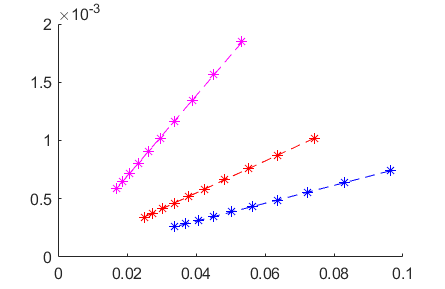
\includegraphics[width=0.4\linewidth]{L2Kc}
\caption{拟合结果。横轴:$(1-2L_2)^2$,纵轴:$K_c$}
\label{fn2}
\end{figure}


\subsection*{$L_4$和$A_c$之间的关系}

进一步分析发现,如果$N_4$等于$0$,模型中就不会出现相变。在$N_4$靠近0的时候,相变点会不断变大,直到无穷,此时$A_c$趋于0,所以模型一定要过原点。

我们猜测$L_4$和$A_c$之间的关系为
$$ A_c = B_c L_4 $$

在$N_4$很大的时候,相变会消失,也就是随着$L_4$的增大,$1/K_c$会在某个有限的位置趋于无穷。因此这里得到的关系只有在$L_4$较小的某个范围内才成立。

在以下三组参数对模型进行拟合,得到拟合的参数值和$R^2$如下:
\begin{align*}
N=(5, 2(11+n), 3, n, 3), \quad n \in [0.4, 1.6], \quad B_c = 0.0129, \quad R^2 = 1 - 1.4 \times 10^{-3} \quad \text{图中紫色} \\
N=(6, 2(14+n), 4, n, 4), \quad n \in [0.4, 1.8], \quad B_c = 0.0071, \quad R^2 = 1 - 8.6 \times 10^{-4} \quad \text{图中红色} \\
N=(7, 2(17+n), 5, n, 5), \quad n \in [0.4, 2.1], \quad B_c = 0.0052, \quad R^2 = 1 - 1.2 \times 10^{-3} \quad \text{图中蓝色}
\end{align*}

图\ref{fn4}中可以看出,拟合结果比较好。
\begin{figure}[h]
\centering
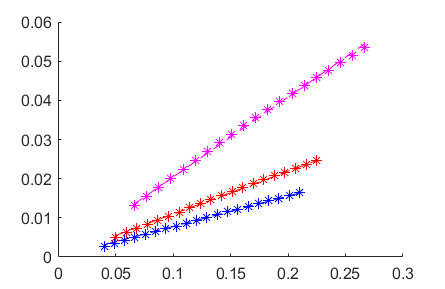
\includegraphics[width=0.4\linewidth]{L4Ac}
\caption{拟合结果。横轴:$L_4$,纵轴:$A_c$}
\label{fn4}
\end{figure}

\subsection*{$L_1$和$B_c$之间的关系}

进一步分析发现,如果$N_1$等于$\max\{N_3,N_5\}$,模型中就不会出现相变。在$N_1$趋近于$\max\{N_3,N_5\}$的时候,相变点会不断变大,直到无穷,此时$B_c$趋于0,所以模型一定要过原点。

同样的,随着$L_1$的增大,$1/K_c$会在某个有限的位置趋于无穷。因此这里得到的关系只有在$L_1$较小时成立。

我们猜测在$0.5 < L_1 < 0.75$区间内,它和$K_c$之间的关系为
$$ \log(B_c) = D_c (L_1 - 0.5) + E_c $$
这个模型既不过原点,也不在有限点处趋于无穷,但是它是目前区间内和数据拟合效果最好的模型。

在以下三组参数对模型进行拟合,得到拟合的参数值和$R^2$如下:
\begin{align*}
N=(n, 2(7+n), 3, 1, 3), \quad n \in [3.5, 4.5], \quad D_c = 7.3358, \quad E_c = -4.0118, \quad R^2 = 1 - 0.0024 \quad \text{图中紫色} \\
N=(n, 2(9+n), 4, 1, 4), \quad n \in [4.5, 6.0], \quad D_c = 7.7312, \quad E_c = -4.1023, \quad R^2 = 1 - 0.006 \quad \text{图中红色} \\
N=(n, 2(11+n), 5, 1, 5), \quad n \in [5.5, 7.5], \quad D_c = 8.0747, \quad E_c = -4.1830, \quad R^2 = 1 - 0.010 \quad \text{图中蓝色}
\end{align*}

图\ref{fn1}中可以看出,拟合结果比较好。由于已经消除了前两个变量的影响,这里的线看起来是重合的。
\begin{figure}[h]
\centering
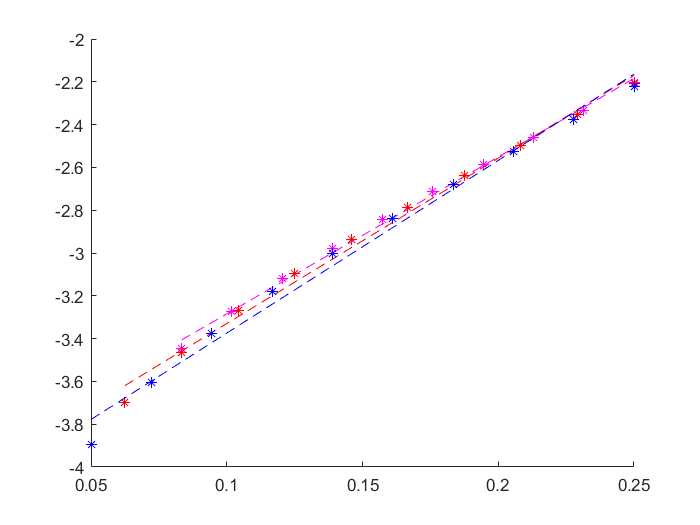
\includegraphics[width=0.4\linewidth]{L1Bc}
\caption{拟合结果。横轴:$L_1 - 0.5$,纵轴:$\log(B_c)$}
\label{fn1}
\end{figure}

\subsection*{总结}

综上所述,得到总的公式为
$$ \frac{1}{K_c} = (1-2L_2)^2 L_4 e^{D_c(L_1 - 0.5) - E_c} $$

在一定范围内取很多点,验证公式的准确性。各项参数的范围是:
\begin{align*}
N_3 & \in [3, 6], \\
N_1 & \in [N3+0.5, 1.5 N3],\\
N_4 & \in [0.5, N_3/2], \\
N_2 & \in [2(N_1+N_3+N_4+N_3), 3(N_1+N_3+N_4+N_3)]
\end{align*}

图\ref{fna}中可以看出,拟合结果比较好,预测值和实际值大致相等。(图中取$D_c=7.1, E_c=4$)
\begin{figure}[h]
\centering
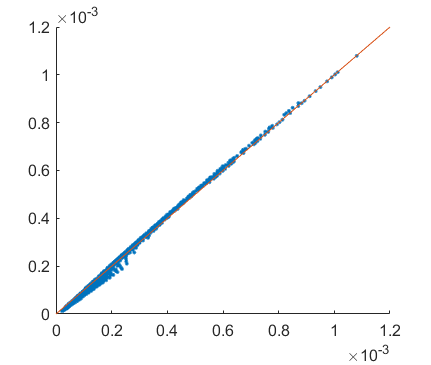
\includegraphics[width=0.4\linewidth]{LaKc}
\caption{拟合结果。横轴:$\frac{1}{K_c}$预测值,纵轴:$\frac{1}{K_c}$模拟值,红线为直线$x=y$}
\label{fna}
\end{figure}


\end{document}